%
% Einfache LaTeX-Vorlage f�r Arbeiten am Lehrstuhl Kranzlm�ller / MNM-Team
% - optimiert f�r die Arbeit mit g�ngigen LaTeX-Editoren
% - funktioniert ohne Makefile und Anpassungen der LaTeX-Verzeichnisstruktur
% - verwendet Komaskript f�r ein (nach europ�ischen Gepflogenheiten) sch�neres Layout
% 
% v1, 2007 (Michael Brenner)
% Diese Version: v1.1, 2012 (Michael Brenner)
% Diese Version: v1.2, 2017 (Michael Brenner)
% 


\documentclass[bibliography=totoc,listof=totoc,BCOR=5mm,DIV=12]{scrbook} % Rand f�r Bindung: 5mm / falls Index verwendet, erg�nze "index=totoc" zu den Optionen 
\usepackage[latin1]{inputenc} % Umlaute im Text
\usepackage{graphicx} % Einf�gen von Grafiken  - f�r PDF-Latex: .pdf und .png (.jpg m�glich, sollte aber vermieden werden)
\usepackage{url}           % URL's (z.B. in Literatur) sch�ner formatieren
\usepackage{hyperref} % sorgt f�r f�r Hyperlinks in PDF-Dokumenten
\usepackage{color}

\graphicspath{{./Bilder/}}

%
% der Befehl \hypenation versteht keine Sonderzeichen, also weder �
% noch "a noch \"a. W�rter die derartige Zeichen enthalten m�ssen
% direkt im Text getrennt werden, z.B. W�r\-ter
%
\hyphenation{Ma-nage-ment}
\hyphenation{Ma-nage-ment-agent}
\hyphenation{Ma-nage-ment-agent-en}
\hyphenation{Ma-nage-ment-ar-chi-tek-tur}
\hyphenation{Ma-nage-ment-ar-chi-tek-tu-ren}
\hyphenation{Ma-nage-ment-an-wen-dung}
\hyphenation{Ma-nage-ment-an-wen-dung-en}
\hyphenation{Ma-nage-ment-an-for-der-ung}
\hyphenation{Ma-nage-ment-funk-ti-on}
\hyphenation{Ma-nage-ment-funk-ti-onen}
\hyphenation{Ma-nage-ment-kon-zep-te}
\hyphenation{Ma-nage-ment-res-source}
\hyphenation{Ma-nage-ment-in-for-ma-ti-on}
\hyphenation{Ma-nage-ment-res-sour-cen}
\hyphenation{ma-nage-ment-re-le-vante}
\hyphenation{ma-nage-ment-sy-stem}
\hyphenation{ma-nage-ment-sy-steme}
\hyphenation{Ma-nage-ment-in-stru-men-tie-rung}
\hyphenation{Ma-nage-ment-platt-form}
\hyphenation{Sys-te-men}
\hyphenation{Sys-tem-um-ge-bun-gen}
\hyphenation{Sys-tem-ma-nage-ment}
\hyphenation{DHCP}
\hyphenation{Ma-nage-ment-diszi-plinen}
\hyphenation{System-management-architekturen}
\hyphenation{Verwendungs-nachweise}
\hyphenation{Video-einricht-ungen}
\hyphenation{Res-source}
\hyphenation{Res-sourcen}
\hyphenation{Grund-anwendung}
\hyphenation{Grund-anwendungen}
\hyphenation{Basis-anwendung}
\hyphenation{Core}
\hyphenation{Kom-mu-ni-ka-ti-on}
\hyphenation{De-sign-ent-schei-dung}
\hyphenation{Sprung-ad-res-sen}
\hyphenation{Klas-si-fi-ka-ti-on}
\hyphenation{Schreib-recht}
\hyphenation{Be-nut-zer-zer-ti-fi-kat}
\hyphenation{Bau-stein-ent-wi-ckler}
\hyphenation{ad-mi-ni-stra-ti-ve}

 % in dieses File kommen W�rter die Latex nicht richtig trennt

\begin{document}

% ---------------------------------------------------------------
\frontmatter % Titelbl�tter und Erkl�rung jeweils spezifisch f�r die jeweilige Uni einbinden
    %%%%%%%%%%%%%%%%%%%%%%%%%%%%%%%
% erste Seite

\thispagestyle{empty}

\begin{center}

\vspace*{-2cm}

{\Huge INSTITUT F�R INFORMATIK\\[1mm]}
DER LUDWIG--MAXIMILIANS--UNIVERSIT�T M�NCHEN\\

\vspace*{1cm}


\includegraphics[width=0.3\textwidth]{lmu_siegel}

\vspace*{2cm}

{\Large \textbf{Master's Thesis}}\\ % oder Fortgeschrittenenpraktikum, Master's Thesis, Bachelorarbeit etc.

\vspace{2.0cm}
{\Huge \textbf{C++ Graph Concepts for}}\\
\vspace*{3mm}
{\Huge \textbf{Partitioned Global Address Space}}\\
\vspace*{20mm}

{\LARGE Stefan Effenberger} % Name des Autors

\vspace{3cm}
\end{center}

\newpage

%%%%%%%%%%%%%%%%%%%%%%%%%%%%%%%
% zweite Seite

\thispagestyle{empty}
\cleardoublepage

%%%%%%%%%%%%%%%%%%%%%%%%%%%%%%%
% dritte Seite (Kopie der ersten)

\thispagestyle{empty}

\begin{center}

\vspace*{-2cm}

{\Huge INSTITUT F�R INFORMATIK\\[1mm]}
DER LUDWIG--MAXIMILIANS--UNIVERSIT�T M�NCHEN\\

\vspace*{1cm}


\includegraphics[width=0.3\textwidth]{lmu_siegel}

\vspace*{2cm}

{\Large \textbf{Master's Thesis}}\\ % oder Fortgeschrittenenpraktikum, SEP etc.

\vspace{2.0cm}
{\Huge \textbf{C++ Graph Concepts for}}\\
\vspace*{3mm}
{\Huge \textbf{Partitioned Global Address Space}}\\
\vspace*{20mm}

{\LARGE Stefan Effenberger} % Name des Autors
\vspace{2cm}

\parbox{1cm}{
\begin{large}
\begin{tabbing}
Aufgabensteller: \hspace{.5cm} \=Prof. Dr. Dieter Kranzlm�ller\\[2mm]
Betreuer:
\>Tobias Fuchs\\[5mm]
Abgabetermin: \> \textcolor{red}{ADD DATE}\\
\end{tabbing}
\end{large}}\\
\vspace{5mm}

\end{center}
 % Titelbl�tter LMU - auskommentieren falls TUM-Arbeit
%    % Richtlinien, siehe http://wwwpa.in.tum.de/generell/Abschlussarbeitsform.html
%
%%%%%%%%%%%%%%%%%%%%%%%%%%%%%%%


% Deckblatt

\thispagestyle{empty}

\begin{center}
    
\includegraphics[width=3cm]{tum-logo}\\
    \vspace{.5cm}
% "Technische Universit�t M�nchen" oder alternativ das Logo der TUM
    {\Large \sc Technische Universit�t M�nchen}\\

    \vspace{1cm}
% "Fakult�t f�r Informatik"
    {\Huge \sc Fakult�t f�r Informatik\\[1mm]}


    \vspace{2cm}
% Diplomarbeit | Master's Thesis | Bachelorarbeit in Informatik | Wirtschaftsinformatik |
    {\Large \textbf{Masterarbeit in Informatik}}\\
% Thema bzw. Titel der Arbeit  (In der Sprache, in der die Arbeit verfasst wurde)
    \vspace{2.0cm}
    {\Huge \textbf{Ein Lorem-Rahmenwerk}}\\ % bei langen Titeln ggf. Schriftgr��e auf \huge herunter setzen
    \vspace*{3mm}
    {\Huge \textbf{f�r Ipsum-Systeme}}\\
    \vspace*{3mm}
    {\Huge \textbf{-- ein Dolor-Ansatz}}\\
    \vspace{1.5cm}
% Vorname und Nachname des Bearbeiters/ der Bearbeiterin
    Vorname Nachname

    \vspace{5cm} % ggf. je nach Zeilenzahl und Schriftgr��e des Titels anpassen
    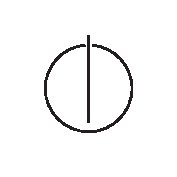
\includegraphics[width=2.4cm]{tum-info-logo}
\end{center}

\newpage

%%%%%%%%%%%%%%%%%%%%%%%%%%%%%%%
% R�ckseite Deckblatt

\thispagestyle{empty}
\cleardoublepage

%%%%%%%%%%%%%%%%%%%%%%%%%%%%%%%
% Erste Seite (Titelblatt)

\thispagestyle{empty}

\begin{center}

    
\includegraphics[width=3cm]{tum-logo}\\
    \vspace{.5cm}
    {\Large \sc Technische Universit�t M�nchen}\\


    \vspace{.5cm}

    {\huge \sc Fakult�t f�r Informatik\\[1mm]}


    \vspace{1cm}

    {\Large \textbf{Diplomarbeit in Informatik}}\\ % oder SEP etc.

% Thema bzw. Titel der Arbeit  (In der Sprache, in der die Arbeit verfasst wurde)
    \vspace{1.5cm}
    {\huge \textbf{Ein Lorem-Rahmenwerk}}\\ % bei langen Titeln ggf. Schriftgr��e herunter setzen
    \vspace*{3mm}
    {\huge \textbf{f�r Ipsum-Systeme}}\\
    \vspace*{3mm}
    {\huge \textbf{-- ein Dolor-Ansatz}}\\

% die englische bzw. deutsche Entsprechung des Titels
    \vspace{1cm}
    {\huge \textbf{A Lorem Framework}}\\ % bei langen Titeln ggf. Schriftgr��e herunter setzen
    \vspace*{3mm}
    {\huge \textbf{for Ipsum Systems}}\\
    \vspace*{3mm}
    {\huge \textbf{-- a Dolor Approach}}\\
    \vspace{1cm}

    \parbox{1cm}{
      \begin{large}
        \begin{tabbing}
          Bearbeiter: \hspace{1.5cm}
            \=Vorname Nachname\\[2mm]
    Aufgabensteller: \>Prof. Dr. Dieter Kranzlm�ller\\[2mm]
    Betreuer: \>MNM-Team-Betreuer 1\\ % alphabetische Reihenfolge (Nachname)
    \>MNM-Team-Betreuer 2\\
    \>Externer Betreuer 1 (Firma)\\[5mm]
    Abgabedatum: \> 7. Juli 2077\\
        \end{tabbing}
      \end{large}
    }\\

    \vspace{.3cm}

    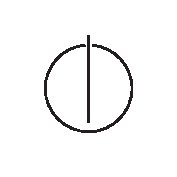
\includegraphics[width=2.4cm]{tum-info-logo}

\end{center}
 % Titelbl�tter TUM - auskommentiert lassen falls LMU-Arbeit
    \thispagestyle{empty}
    \cleardoublepage
    %
% LaTeX-Rahmen f�r Arbeiten am Lehrstuhl Hegering
%
% Harald Roelle, 2001, 2002
%
% basierend auf Arbeiten von Helmut Reiser, Boris Gruschke und Stephen Heilbronner
%

\newpage

\thispagestyle{empty}

\begin{large}

\vspace*{2cm}

\noindent
Hiermit versichere ich, dass ich die vorliegende Masterarbeit
selbst�ndig verfasst und keine anderen als die angegebenen Quellen
und Hilfsmittel verwendet habe.

\vspace{2cm}

\noindent
M�nchen, den \textcolor{red}{ADD DATE}

\vspace{3cm}

\hspace*{7cm}%
\dotfill\\
\hspace*{8.5cm}%
\textit{(Unterschrift des Kandidaten)}

\end{large}
 % Erkl�rung (Arbeit selbstst�ndig verfasst) - auskommentieren falls TUM-Arbeit
%    \begin{large}

\vspace*{2cm}
\noindent
Ich versichere, dass ich diese Masterarbeit % (bzw. Master's Thesis)
selbst�ndig verfasst und nur die angegebenen Quellen und Hilfsmittel verwendet habe.

\vspace{2cm}

\noindent
M�nchen, den 7. Juli 2077

\vspace{3cm}

\hspace*{7cm}%
\dotfill\\
\hspace*{8.5cm}%
\textit{(Unterschrift des Kandidaten)}

\end{large}
 % Erkl�rung (Arbeit selbstst�ndig verfasst) - auskommentiert lassen falls LMU-Arbeit
    \thispagestyle{empty}
    \cleardoublepage
    \vspace*{2cm}

\begin{center}
    \textbf{Abstract}
\end{center}

\vspace*{1cm}

\noindent Hier steht eine kurze Zusammenfassung der Arbeit. Sie darf auf gar keinen Fall
l�nger als eine Seite sein, ca. eine drittel bis eine halbe Seite ist optimal.

 % Abstract
    \thispagestyle{empty}
    \tableofcontents % Inhaltsverzeichnis

% ---------------------------------------------------------------
\mainmatter % die eigentliche Arbeit

\chapter{Introduction}
Many scientific projects are largely enabled by simulation. Because such simulations often require huge computational capabilites, single compute nodes with a shared-memory architecture cannot provide enough computation power and storage for numerous cases. For this reason, in High Performance Computing (HPC), work is distributed among multiple, interconnected nodes to facilitate the solving of large problems in a timely manner. Since processors cannot directly access the memory of other nodes, the traditional programming model for such systems requires programmers to explicitly distribute data between nodes via message passing. This imposes high demands on the programming skills of scientists who might not have a background in computer science.

Therefore, with the Partitioned Global Address Space (PGAS) model, a new approach is proposed: The memory space of individual nodes in a system is unified within a global address space so that each node can directly access the memory of all other nodes. Programmers are still required to keep data access between nodes to a minimum because data transferal over an interconnect is costly. To further reduce the demands on the programmer, distributed data structures that handle data distribution and load balancing are needed.

Furthermore, data-intensive tasks have been gaining a continually growing interest in the scientific community. Traditionally, applications in HPC follow a computation-centric approach by solving numerical algorithms in the fastest possible way. As ``Big Data'' is becoming increasingly important in scientific projects, a shift towards more data-oriented applications can be observed in recent HPC projects \cite{fusionfs}. This trend requires distributed data structures that allow for the storage of large amounts of irregular data and cater to the needs of ever-changing dynamic data.

\section{Problem statement}
Data can be represented in numerous ways. The most generic form of data representation is enabled by \textit{graphs}. A graph G(V, E) is a pair with a set of vertices V and a set of edges E that connect the vertices. This allows for the representation of data and its relationships in regular as well as irregular patterns.

On distributed machines, graph data structures can be implemented using a variety of different characteristics. This has lead to many different implementations - usually a new implementation for each algorithm - which are hardly compatible with each other. To overcome this situation, generic programming abstractions to facilitate reuse of existing code and to lower the demands on programmers are needed.

As of today, no generic graph abstractions implementing the PGAS model exist. This work therefore aims to provide a graph abstraction for C++ containers that allows for the implementation of arbitrary graph algorithms following the PGAS model on distributed memory machines.

\section{Scope and Objectives}
In this work, a C++ concept for graph containers following the PGAS model is presented. The concept is part of the DASH C++ Template Library and thus uses concepts already present in the library. 

The graph concept is meant to provide a generic framework for the programming of arbitrary graph algorithms in the context of distributed machines and especially the Partitioned Global Address Space model. This means that it meets the following requirements:

\begin{itemize}  
\item Native support for one-sided communication
\item Support for the programming of synchronous graph algorithms
\item Support for the programming of asynchronous graph algorithms
\item Portability across platforms (\textcolor{red}{PORTABLE EFFICIENCY?})
\item Support for heterogenous systems
\item \textcolor{red}{FINISH REQUIREMENTS}
\end{itemize}

Furthermore, this work provides concepts for the dynamic allocation of graph data across multiple machines with a focus on optimized data locality. \textcolor{red}{LOAD BALANCING?}

A reference implementation is then used to verify the usability, correctness and universality of the given concepts. While the concepts are designed for high performance, the reference implementation is not. This means that the evaluation of this implementation does not account for the performance of this work's concepts.

\chapter{Background}
This chapter covers some fundamental background knowledge needed for a better understanding of the following chapters of this thesis. Only explanations directly relevant to the topics of this thesis are provided.

Since the result of this work is a C++ concept, some important language expressions and concepts are firstly discussed, along with a description of the Standard Template Library on which concepts this work is built upon. The reader is then introduced to the domain of High Performance Computing which is the main application area for this work. A brief overview of the Partitioned Global Address Space programming model is then followed by a description of the DASH Library which provides core concepts used in this thesis.

\section{C++ Concepts}
The graph concepts of this work are part of the DASH C++ Template Library (see \autoref{dash_section}). For this reason, the reference implementation is written in C++11 \cite{c++11}. This section illustrates some basic knowledge about important C++ concepts used in the implementation description of \autoref{impl_section}.

\subsection{Language Concepts}
\subsubsection{Value and referential semantics}
%copy elision
\subsubsection{Operator Overloading}
\subsubsection{Const correctness}
\subsubsection{Static polymorphism}
\subsubsection{Resource Acquisition Is Initialization}
\subsubsection{Rule of three/five/zero}

\subsection{Standard Template Library}
\subsubsection{Concepts}
\subsubsection{Iterators}
\subsubsection{Containers}


\section{High Performance Computing}
\label{hpc_section}
High Performance Computing (HPC) is a broad term describing advances for the fastest possible computation of a given problem. Gustafson's Law \cite{gustafson} suggests that a compute system can linearly grow with the problem size: A problem of two times its original size can be computed on a system with twice as many processors in the same time (best case scenario). This means that very large problems can be computed in an acceptable timeframe if there is a sufficiently large compute system available. Depending on the problem size, two different system architectures are used in HPC:

\paragraph{Shared Memory}
A shared memory system consists of a single node with multiple processors connected to the same random access memory. Memory access for the different processors can be uniform, but many systems implement a non-uniform memory access (NUMA) design where a part of the memory is assigned to each of the processors. A processor in a NUMA system can access its assigned memory faster than the memory of the other processors.
Because processors can access all data at all times, communication between processors has a low cost which simplifies programming on these systems in comparison to distributed memory systems. Achieving high performance on NUMA systems is more problematic because the programmer has to take data locality into account \cite{numa}.

\paragraph{Distributed Memory}
Multi-processor systems in which each processor has access to its own memory space are called distributed memory systems. These systems usually consist of several shared memory nodes with the processors of one node not being able to directly access memory of other nodes. While single shared memory systems can only be scaled to a certain extent, the scalability of distributed systems is much higher \cite{dismem}.

The nodes are connected with a network interconnect for communication between the processors. Due to the latency of the interconnect being significantly higher than the latency of a memory bus in a shared memory system, communication is much more costly. This imposes higher demands on the programmers' skills in comparison to shared memory systems.\\

The largest problems in science are computed on ``supercomputers'' like the \textit{SuperMUC} at the \textit{Leibniz Rechenzentrum} in Munich. These distributed memory machines consist of hundreds or even thousands of homogeneous nodes that are connected with a specialized interconnect. To this date, \textit{message passing} is the prevalent programming model for such systems.

\section{Partitioned Global Address Space}
\textit{Shared Memory} and \textit{Message Passing} are the dominant models in HPC as of this writing. As pointed out in \autoref{hpc_section} however, the usage of Message Passing requires high skills in computer architecture and programming. To ease this problem, the Partitioned Global Address Space (PGAS) model has been proposed. It unifies some of the benefits of both of these models by creating a global address space over the initially local-only address spaces of distributed machines.\\

\autoref{pgas_figure} a) presents the architecture of a shared-memory machine: Multiple processors share a common address space. The processors are attached to the same memory over a bus. In some systems, memory might be local to some processors which means the rest of the processors has a higher latency when trying to access the non-local memory. Still, every processor can access every part of the address space. Communication takes place \textit{implicitly} by writing and reading shared variables.  Because data written by one processor can be accessed by another processor in a fast manner, little care has to be taken regarding the decomposition of data. For this reason however, shared memory programs are typically not scalable on distributed machines \cite{apgas}.\\

\autoref{pgas_figure} b) shows that a distributed memory machine basically consists of several shared memory machines linked to each other via an interconnect. Since processors cannot directly access data stored in the memory of other machines, \textit{explicit communication} is needed in order to synchronize the processors. This is typically done by two-sided communication: The \textit{sending} of a message has to be accepted at the remote machine with a a corresponding \textit{receive} call. 

Machines conduct their computations simultaneously and either synchronize in discrete time intervals or exchange data asynchronously. Either way, sending data over an interconnect imposes high latency and low throughput in comparison to the data access over a memory bus in shared memory systems. For this reason, programmers have to carefully decompose data in order to distribute the work load uniformly and minimize communication overhead.\\

\autoref{pgas_figure} c) illustrates the concept of Partitioned Global Address Space: The local portions of memory are unified under a global address space which allows processors to directly access data on remote machines. Data access is performed using one-sided communication: No \textit{receive} call on the remote machine is needed. 

Since data transferal over an interconnect is still costly, programmers have to take the same care for data locality as with the traditional message passing approach. To allow for this, the locality of a datum is directly exposed to the programmer.

\begin{figure}[ht]
	\centering
  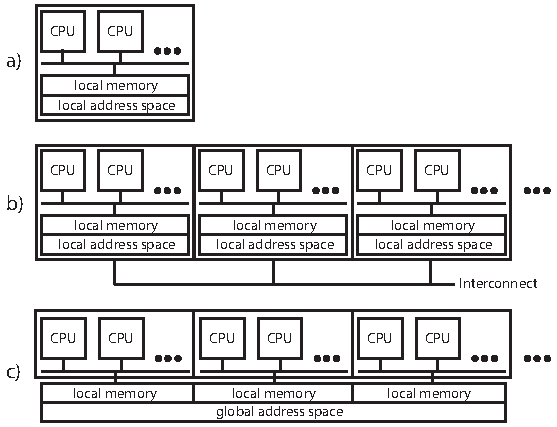
\includegraphics[width=1\textwidth]{Bilder/pgas.pdf}
	\caption{View on a) Shared Memory b) Distributed Memory c) Partitioned Global Address Space}
	\label{pgas_figure}
\end{figure}

Existing PGAS approaches are mainly comprised of dedicated programming languages such as Unified Parallel C (UPC) \cite{upc}, Co-Array Fortran \cite{co_array_fortran} or Chapel \cite{chapel} that allow for compiler optimizations in respect to distributed machines but lack portability and reach. In contrast to this, efforts exist to create libraries for existing programming languages used by many HPC systems.

\section{DASH C++ Template Library}
\label{dash_section}
DASH \cite{dash} is a compiler-free PGAS approach: It consists of a simple C++ library that can be compiled with any C++ compiler and thus can be used out-of-the-box on most HPC systems. The library is part of the Priority Programme ``Software for Exascale Computing'' (SPPEXA)\footnote[1]{http://www.sppexa.de} which supports research on computing systems achieving $10^{18}$ floating point operations per second and above. While PGAS languages require existing programs to be completely rewritten from scratch, DASH allows the applications to be incrementally ported and thus facilitates wider adoption of the PGAS model in the HPC community.

DASH operates on top of the \textit{DASH Runtime} (DART) which is a PGAS memory allocation and communication abstraction written in C. DART enables global memory allocation, pointers to remote memory locations and one-sided communication on top of existing libraries like MPI \cite{mpi3} or GASPI \cite{gaspi}. With DART-MPI \cite{dart_mpi}, a fully functional DART abstraction on top of MPI-3 is used in DASH releases at the time of this writing.

In DASH, processing elements are referred to as \textit{units}. Units can be any processing element such as threads or processes. DASH programs are implemented using the Single Program Multiple Data (SPMD) model: The data is partitioned onto the participating units and each unit executes the same code on its part of the data. Furthermore, units  form \textit{teams} that can be created at runtime. Because HPC hardware topologies become more complex over time (e.g. \cite{dragonfly}), DASH supports hierarchical team creation to allow for a more fine-grained exploitation of data locality compared to the typical local-remote distinction of the PGAS model.

Data is referred to in terms of global pointers and references. A \texttt{GlobPtr<T>} object holds information about the unit and local memory location of the referenced datum. It can be dereferenced to a \texttt{GlobRef<T>} object which behaves like a C++ reference and can be converted to an object of type \texttt{T}. This type conversion triggers a one-sided get operation transferring the data from its remote source to the caller. Similarly, data can be written into the referenced memory location of a \texttt{GlobRef<T>} object.

DASH provides a set of containers for distributed data storage. Aside from the static data structures Array and Matrix, dynamic data structures are available. Since the graph concepts of this work belong into the latter category, details of it are discussed in the following.\\

Dynamic allocation in DASH is encapsulated in the \texttt{GlobHeapMem} concept. \texttt{GlobHeapMem} offers two basic operations to dynamically allocate memory during runtime: \texttt{grow} and \texttt{shrink}. These operations increase or decrease the local size of the memory allocated on the respective unit. Changes in memory space are not reflected in global address space until the operation \texttt{commit} is called which publishes the changes across all units.

A dynamic container in DASH pre-allocates some memory during its initialization. When the  memory is completely used, further additions of elements result in \texttt{GlobHeapMem.grow} operations. A call to the \texttt{barrier} operation of the container results in all newly added elements of the container to be publicly available on all units.

\chapter{Related Work}
\section{Shared Memory}
\subsection{STINGER}
\subsection{Ligra}
\section{Distributed Memory}
\subsection{Parallel Boost Graph Library}
\subsection{STAPL Parallel Graph Library}

\chapter{Graph Container Concepts}
\section{Memory Space}
\section{Index Space}
\section{Iteration Space}
%http://www.open-std.org/jtc1/sc22/wg21/docs/papers/2011/n3242.pdf ab 718
%hierarchie
\section{Semantics}
%Computational constraints/assumptions

\chapter{Reference Implementation}
\label{impl_section}

\chapter{Case studies}
\section{Static structure}
\subsection{Graph traversal}
\subsection{Shortest path evaluation}
\section{Dynamic Structure}
\subsection{Graph partitioning}
\subsection{De Bruijn Graph construction}

\chapter{Evaluation}
\section{Micro-benchmarks}

\chapter{Conclusion}
\section{Summary}
\section{Assessment}
\section{Outlook}

% ---------------------------------------------------------------
\backmatter % ab hier keine Nummerierung mehr
    \listoffigures
    \bibliographystyle{alphadin}
    \bibliography{./Bib/effe17}

\end{document}
